%&LaTeX

% Sections of this are duplicated from the DSP First labs 1a and
% 1b. Those sections MUST be rewritten before this can be released
% externally.


\section{Complex Exponentials in J-DSP}

% TODO: redo this beginning section to introduce the idea of a time
% series in JDSP relate the rotating phasors addition to moving back
% and forth along the real axis.  Scrap the MATLAB introductions in
% favor of introducing how to look at phasors in JDSP intuitively and
% that the complex plane is just a succinct way of looking at sine
% waves.

In this lab you will be investigating how complex exponentials relate
to sine and cosine waves. Once completed you should have a feel for
how the complex plane can be used to represent \textit{real,
  oscillating functions} (like sines and cosines). Moreover, you
should have an appreciation for why it is easier to mathematically
manipulate and analyze oscillating functions using complex
arithmetic. We will be using J-DSP exclusively to illustrate key
concepts of how complex numbers can represent frequency.

\subsection{Complex Vectors and Exponentials in J-DSP}
\label{sc:jdsp-sines}
In this section you will use J-DSP to generate vectors and phasors in the complex plane. Specifically, you will relate changes in the complex plane to changes in the time domain.

% Complex Vector in J-DSP
\begin{figure}[t]
  \begin{center}
    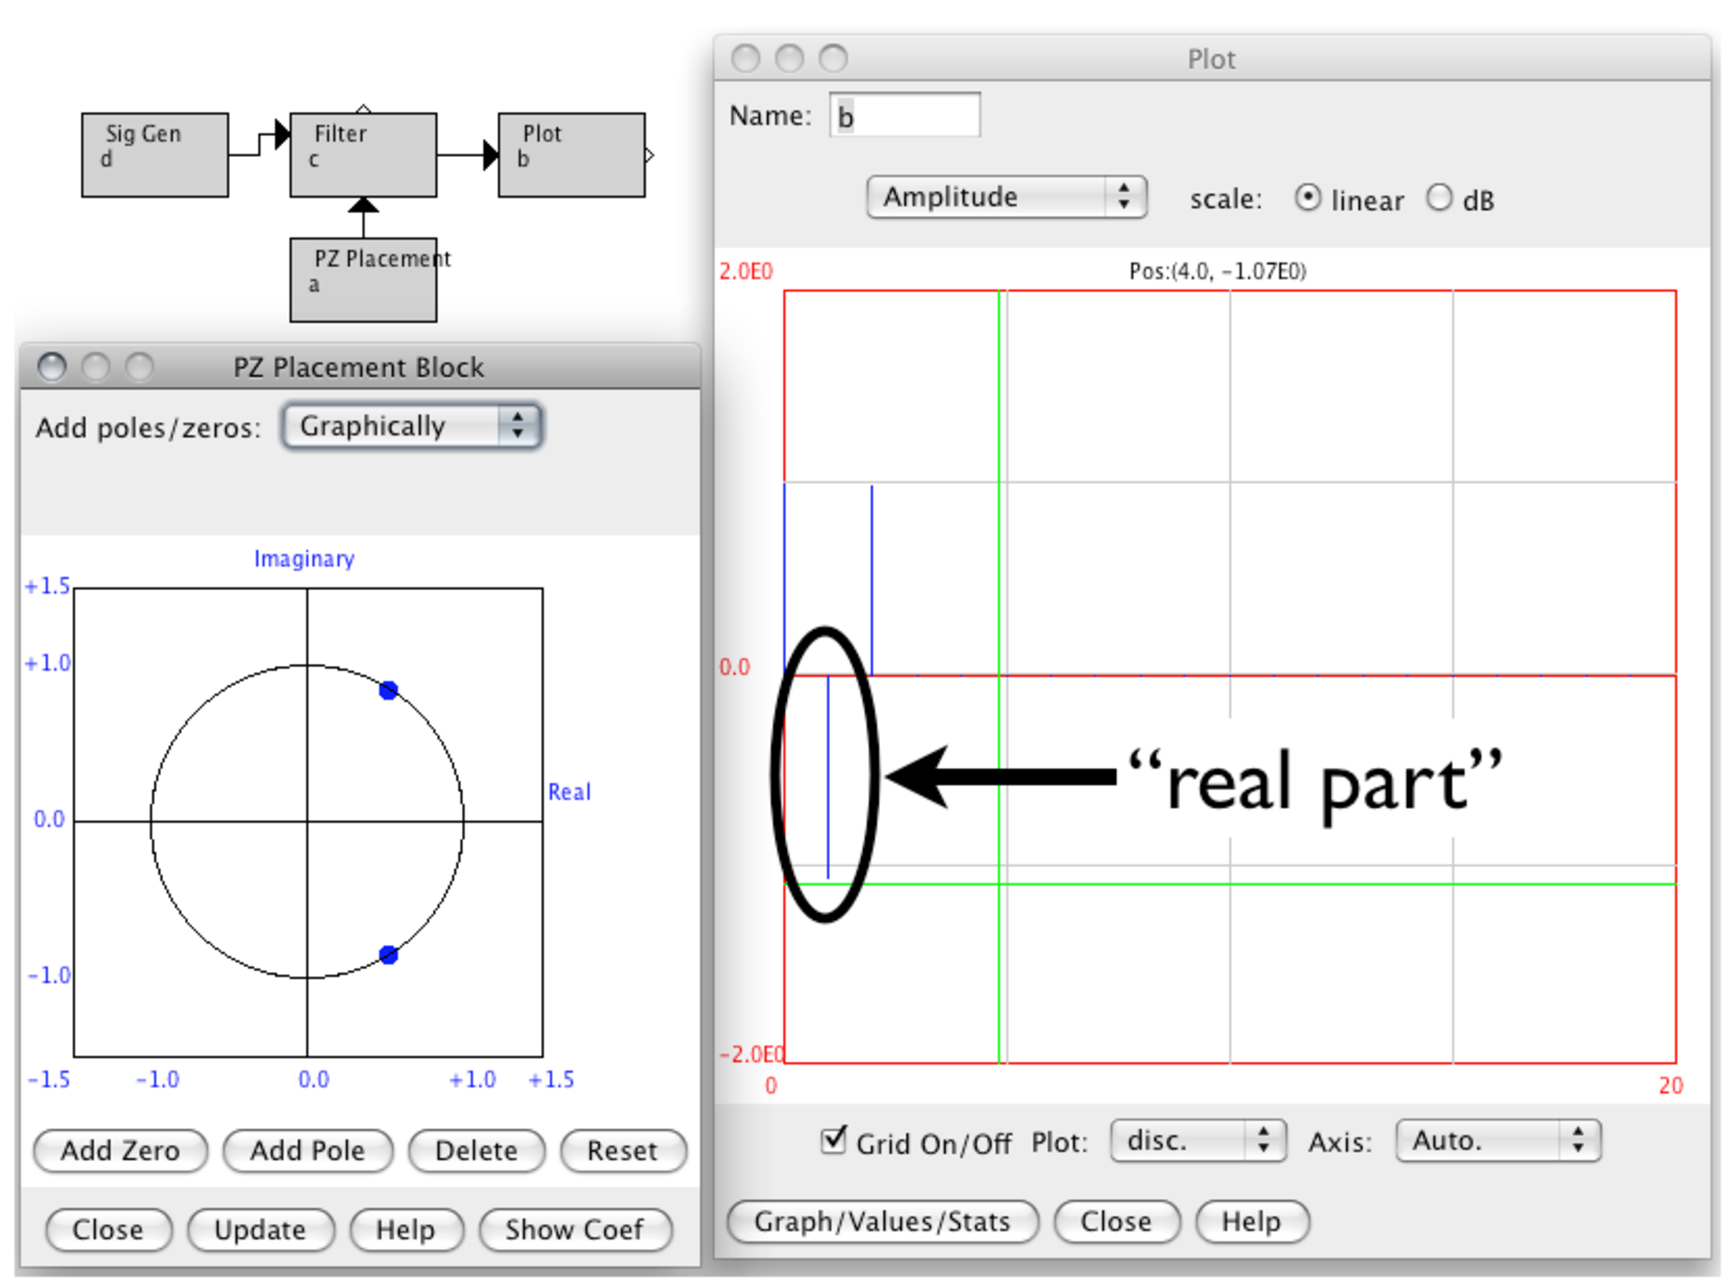
\includegraphics[height=3in]{lab2/PoleZeroAsComplexVector}
  \end{center}
\caption{J-DSP setup for simulating a two vectors that add to be a real output, represented as sample 2 in the plot.\label{fg:PoleZeroAsComplexVec}}
\end{figure}

% idea of the vectors in the complex plane
\paragraph{Step 1.1} 
WARNING: The next step will overwrite any work not saved in J-DSP. Use the given script to generate the diagram in Figure \ref{fg:PoleZeroAsComplexVec}. Download: \url{http://faculty.washington.edu/stiber/pubs/Signal-Computing/jdsp-scripts/polezero_as_vector.txt}.

Use the \menu{File} $\rightarrow$\menu{Import from Script...} command in the J-DSP window and copy the text  over. You should see a block diagram similar to that in Figure \ref{fg:PoleZeroAsComplexVec}. If you do not, there was a failure loading the script, exit out of J-DSP, and try again. 
This script provides an interactive way to \textit{view vectors} in the complex plane and what they look like in the time domain. We are not yet ready to talk about every block in the J-DSP diagram. However, two blocks are of interest to us now. We will interact with \block{PZ-Placement} (block a) and \block{Plot} (block b). Open the dialog for the \block{Plot} block in the diagram if it is not already active. You should see three discrete points in the output plot (Figure \ref{fg:PoleZeroAsComplexVec}). 

Now open the dialog for \block{PZ-Placement} if it is not already active. You should see a plot of the complex plane with two $\circ$ marks on it and a large black circle that represents the unit circle. This \block{PZ-Placement} block is normally used for filter design, but we will be using it to represent a vector in the complex plane, $Re^{j\phi}$. If you drag the $\circ$ marks in \block{PZ-Placement}, you can change the amplitude and phase of the vector and view the ``real part'' of the output in the time domain plot. When you do this, you will also see the three points in the output plot change in magnitude. We will be interested in what happens to the middle value in the plot (marked ``real part'' in Figure \ref{fg:PoleZeroAsComplexVec}). You can (1) click and drag or (2) you can enter the real and complex values manually using the \button{Graphically} and \button{Manually} selections from the pop-up menu. 
Note that the \block{PZ-placement} block is doing more than just helping to plot the ``real part'' of the complex vector. For now, just know that the second point plotted in the \block{Plot} dialog corresponds to the ``real part''  of the complex vector. It is directly affected by the magnitude and phase of the vector. For the following questions, recall that a phasor is just a spinning vector in the complex plane.  

\begin{enumerate}
\item If you repeatedly drag the $\circ$ marks in a circular motion along the black circle in \block{PZ-placement}, what happens to the ``real part'' in the plot dialog? If you were to keep the vector magnitude constant and graph the ``real part'' of the plot over time as it moves around the complex plane, would you expect to see a sinusoidal wave? How would the amplitude and phase of the sinusoidal wave be affected by the complex vector?

\end{enumerate}


% Complex Phasor in J-DSP
\begin{figure}[t]
  \begin{center}
    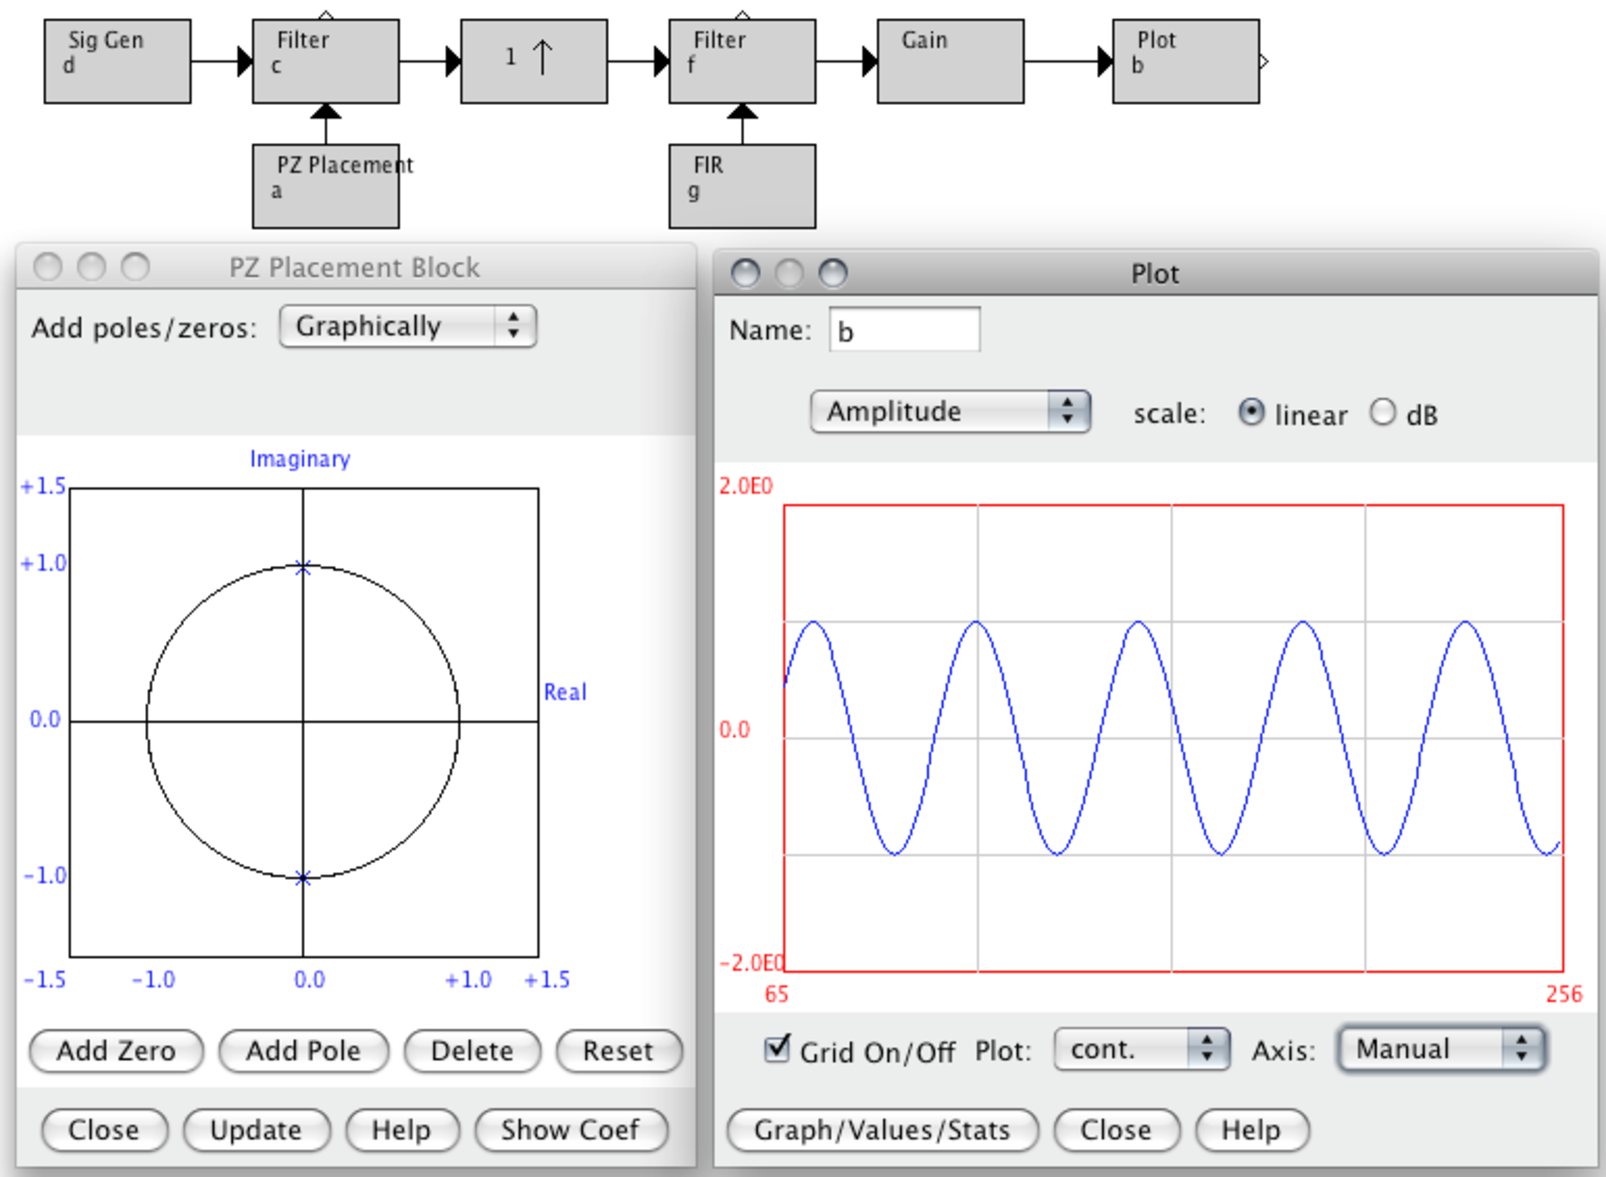
\includegraphics[height=3in]{lab2/PoleZeroAsComplexExp}
  \end{center}
\caption{J-DSP setup for simulating two phasors that add to be a real sinusoid.\label{fg:PoleZeroAsComplexExp}}
\end{figure}

% introduce the pole zero placement as means of visualizing the phasor (only a weak analogy, it would be great to have a built-in J-DSP phasor animation function)
\paragraph{Step 1.2} 
WARNING: The next step will overwrite any work not saved in J-DSP. Use the given script to generate the diagram in Figure \ref{fg:PoleZeroAsComplexExp}. Download: \url{http://faculty.washington.edu/stiber/pubs/Signal-Computing/jdsp-scripts/polezero_as_phasor.txt}. 

Use the \menu{File} $\rightarrow$\menu{Import from Script...} command in the J-DSP window and copy the text  over. You should see a block diagram similar to that in Figure \ref{fg:PoleZeroAsComplexExp}. If you do not, there was a failure loading the script, exit out of J-DSP, and try again. 

This script provides an interactive way to manipulate the \textit{frequency} of phasors in the complex plane and view the sinusoidal output. We are not yet ready to talk about every block in the J-DSP diagram. Like before, two blocks are of interest to us now. We will interact with \block{PZ-Placement} (block a) and \block{Plot} (block b). Open the dialog for the \block{Plot} block in the diagram if it is not already active. You should see a cosine wave. (Note that, in the plot in the figure, the limits of the $X$-axis have been changed manually to have a lower limit of 65, rather than zero. Unfortunately, the axis limits don't get restored when a script is imported, so you will see the auto axis limits, rather than the ones set as in the figure. You can set the limits in the plot to match the figure yourself.)

Now open the dialog for \block{PZ-Placement} if it is not already active. This block is normally used for filter design, but we will be using it to simulate a phasor in the complex plane. Recall that a phasor can be represented in polar form as $Re^{j\omega t}$ where $\omega $ represents the frequency at which the phasor rotates and $R$ represents the magnitude. Dragging the \texttt{x} marks in \block{PZ-Placement} lets you change the $\omega $ of the resulting phasor and view the sinusoid in real time. Note that you can also change the magnitude of the complex phasors in the dialog, but this is not the same as changing the amplitude of a complex phasor. There are other things going on in this block that we are not ready to talk about - we are actually treating something called a ``pole'' as a rotating phasor, which is not quite right. For now, try to keep the magnitude of the phasor as close to ``one'' as possible (i.e., try to keep the \texttt{x} on the black line representing the unit circle). 

\begin{enumerate}
\item Drag the phasors along the unit circle towards the (1,0) point (where the unit circle meets the real axis in the right half plane). What happens? What happens when you move away from the the (1,0) point along the unit circle? Include a screenshot of the \block{Plot} and \block{PZ-placement} dialogs in your lab report.


\item Notice that you cannot move only one of the phasors. You must move both at the same time. Does it make sense that you must move both symmetrically? Why or why not? \textit{Hint:} think about the output as being the rotating phasors $e^{j\omega_1 t}+e^{j\omega_2 t}$, where $\omega_1$ and $\omega_2 $ are proportional to the angles of the ``poles.''

\end{enumerate}


\subsection{Complex Exponentials}

\paragraph{Step 2.1} Compute the following complex arithmetic by hand:
\begin{enumerate}\renewcommand{\theenumi}{\alph{enumi}}
\item What is the complex conjugate of $z_1 = -1 + j 0.3$?

\item Let $z_2 = 1 + j 0.6$ What is $z_1 + z_2$?

\item What is $z_1 - z_2$?

\item What is $z_1 z_2$?

\item What is $z_2/z_1$?

\end{enumerate}

\paragraph{Step 2.2} Compute or prove the following using complex arithmetic and Euler's Formula by hand. Recall that Euler's Formula is given by: $e^{\pm j\omega t}=\cos(\omega t) \pm j \sin(\omega t)$.

\begin{enumerate}
\item A complex number can be written in rectangular coordinates as $z
  = x + j y$. Write the relations to calculate the polar form, $z=(r,
  \theta)$ or $z = r e^{j\theta}$.

\item Using Euler's formula, express $\cos x$ and $\sin x$ as a
  combination of complex exponentials.
  
\item Convert $\cos(\omega t+\phi)$ into the sum of complex exponentials.  

\item Find expressions for 1, $j$, $1 + j$, $(1 + j\sqrt{3})/2$ as
  complex exponentials.

\item Compute $[(1+j\sqrt{3})/2]^2$ and $(1+j)^4$ directly (using the
  rectangular representations).
  
\item Compute $[(1+j\sqrt{3})/2]^2$ and $(1+j)^4$ using complex
  exponentials.
  
\end{enumerate}


\paragraph{Step 2.3} Prove the following regarding complex conjugates:

\begin{enumerate}
\item Show that $(z_xz_y)^* = z_x^* z_y^*$.

\item Express $|z|^2$ as a function of $z$ and $z^*$.

\end{enumerate}




\subsection{Complex Exponentials in J-DSP}

\paragraph{Step 3.1} In this step, you are asked to use JDSP
to create a block diagram capable of synthesize a waveform of the form:
$\cos(2\pi (200) t+\phi_1) + \cos(2\pi (200) t +\phi_1) +\cos(2\pi (200) t+\phi_1) +\cos(2\pi (200) t+\phi_1) $
And plot the output of each cosine wave and their sum. Use the \block{Cont. Signal} and \block{Analog Adder} blocks in the ``Analog Blocks'' function set. Include a screenshot of the block diagram in your writeup. Use this diagram to complete Step 3.2.


\paragraph{Step 3.2} Generate four sinusoids with the following
amplitudes and phases (remember to convert from rad/s to Hz and from radians to degrees):
\begin{align}
x_1(t) &= 5 \cos(2\pi(200)t +0.5\pi) \\
x_2(t) &= 5 \cos(2\pi(200)t - 0.25\pi) \\
x_3(t) &= 5 \cos(2\pi(200)t +0.4\pi) \\
x_4(t) &= 5 \cos(2\pi(200)t - 0.9\pi) 
\end{align}

\begin{enumerate}\renewcommand{\theenumi}{\alph{enumi}}
\item Make a plots of all four signals in J-DSP. 

\item Verify that the phase of all four signals is correct at $t = 0$,
  and also verify that each one has the correct maximum amplitude. Use
  the \block{Analog Plot} blocks.

\item Create the sum sinusoid,
  $x_5(t)=x_1(t)+x_2(t)+x_3(t)+x_4(t)$. Make a plot of $x_5(t)$ over
  the same range of time as used in the last plot. Include your plot in your writeup 
  
\item Using pencil and paper: Express   $x_1(t)$ through $x_4(t)$ as complex exponentials. 
  
	
\item Using pencil and paper: Express   $x_5(t)$ as a sum of complex exponentials. 	


\item Using complex exponentials, express the amplitude and phase of $x_5(t)$ (use pencil and paper with the aide of a graphing calculator, spreadsheet, or MATLAB).


\end{enumerate}



% LocalWords:  MATLAB DSP
